% Figure 1.

% Title
\newcommand\ftitle{Identification of the WASH complex proteome in vivo confirms a
neuronal role in endosomal trafficking}

% Legend
\newcommand\legend{
	(A) The WASH complex is composed of five subunits, Washc1 (WASH1), Washc2
	(FAM21), Washc3 (CCDC53), Washc4 (SWIP), and Washc5 (Strumpellin). Human
	mutations in these components are associated with spastic paraplegia (De Bot et
	al., 2013; Jahic et al., 2015; Valdmanis et al., 2007), Ritscher-Schinzel
	Syndrome (Elliott et al., 2013), and intellectual disability (Assoum et al.,
	2020; Ropers et al., 2011). 
	(B) A BioID2 probe was attached to the c-terminus of WASH1 and expressed under
	the human synapsin-1 (hSyn1) promoter in an AAV construct for in vivo BioID
	(iBioID). iBioID probes (WASH1-BioID2-HA, or negative control solubleBioID2-HA)
	were injected into wild-type mouse brain at P0 and allowed to express for two
	weeks. Subcutaneous biotin injections (24 mg/kg) were administered over seven
	days for biotinylation, and then brains were harvested for isolation and
	purification of biotinylated proteins. LC-MS/MS identified proteins
	significantly enriched in all three replicates of WASH1-BioID2 samples over
	soluble-BioID2 controls. 
	(C) Representative image of WASH1-BioID2-HA expression in a mouse coronal brain
	section (Cx = cortex, Hipp = hippocampus, Thal = thalamus). Scale bar, 1 mm.
	(D) Representative image of WASH1-BioID2-HA expression in mouse cortex (inset
	from C). Individual panels show nuclei (DAPI, blue), AAV construct HA epitope
	(green), and biotinylated proteins (Streptavidin, red). Merged image shows
	colocalization of HA and Streptavidin (yellow). Scale bar, 50 µm. 
	(E) Representative image of WASH1-BioID2-HA expression in mouse hippocampus
	(inset from C). Scale bar, 50 µm.
	(F) Representative image of WASH1-BioID2-HA expression in mouse thalamus (inset
	from C). Scale bar, 50 µm.
	(G) iBioID identified known and unknown proteins interactors of the WASH complex
	in murine neurons. Nodes size represents protein abundance fold-enrichment over
	negative control (range: 3 to 181.7), solid grey edges delineate iBioID
	interactions between the WASHC1 probe (seen in yellow at the center) and
	identified proteins, dashed edges indicate known protein-protein interactions
	from HitPredict database (López et al., 2015). (H-I) Clustergrams of: 
	(H) All five WASH complex proteins identified by iBioID.
	(I) Previously reported WASH interactors (13/174), including the CCC and
	Retriever complexes.
	(J) Endosomal trafficking proteins (23/174 proteins).
	(K) Endocytic proteins (24/174).
	(L) Proteins involved in cytoskeletal regulation (32/174), including Arp2/3
	subunit ARPC5.
	(M) Synaptic proteins (28/174). Clustergrams were annotated by hand and
	cross-referenced with Metascape (Zhou et al., 2019) GO enrichment of WASH1
	proteome constituents over all proteins identified in the BioID experiment.
	}

% The plotting code.
% Arguments: Title, Legend, Figure Name (path).
\begin{figure}
	\begin{fullwidth}
	\centering
        \figuretitle{\ftitle}
	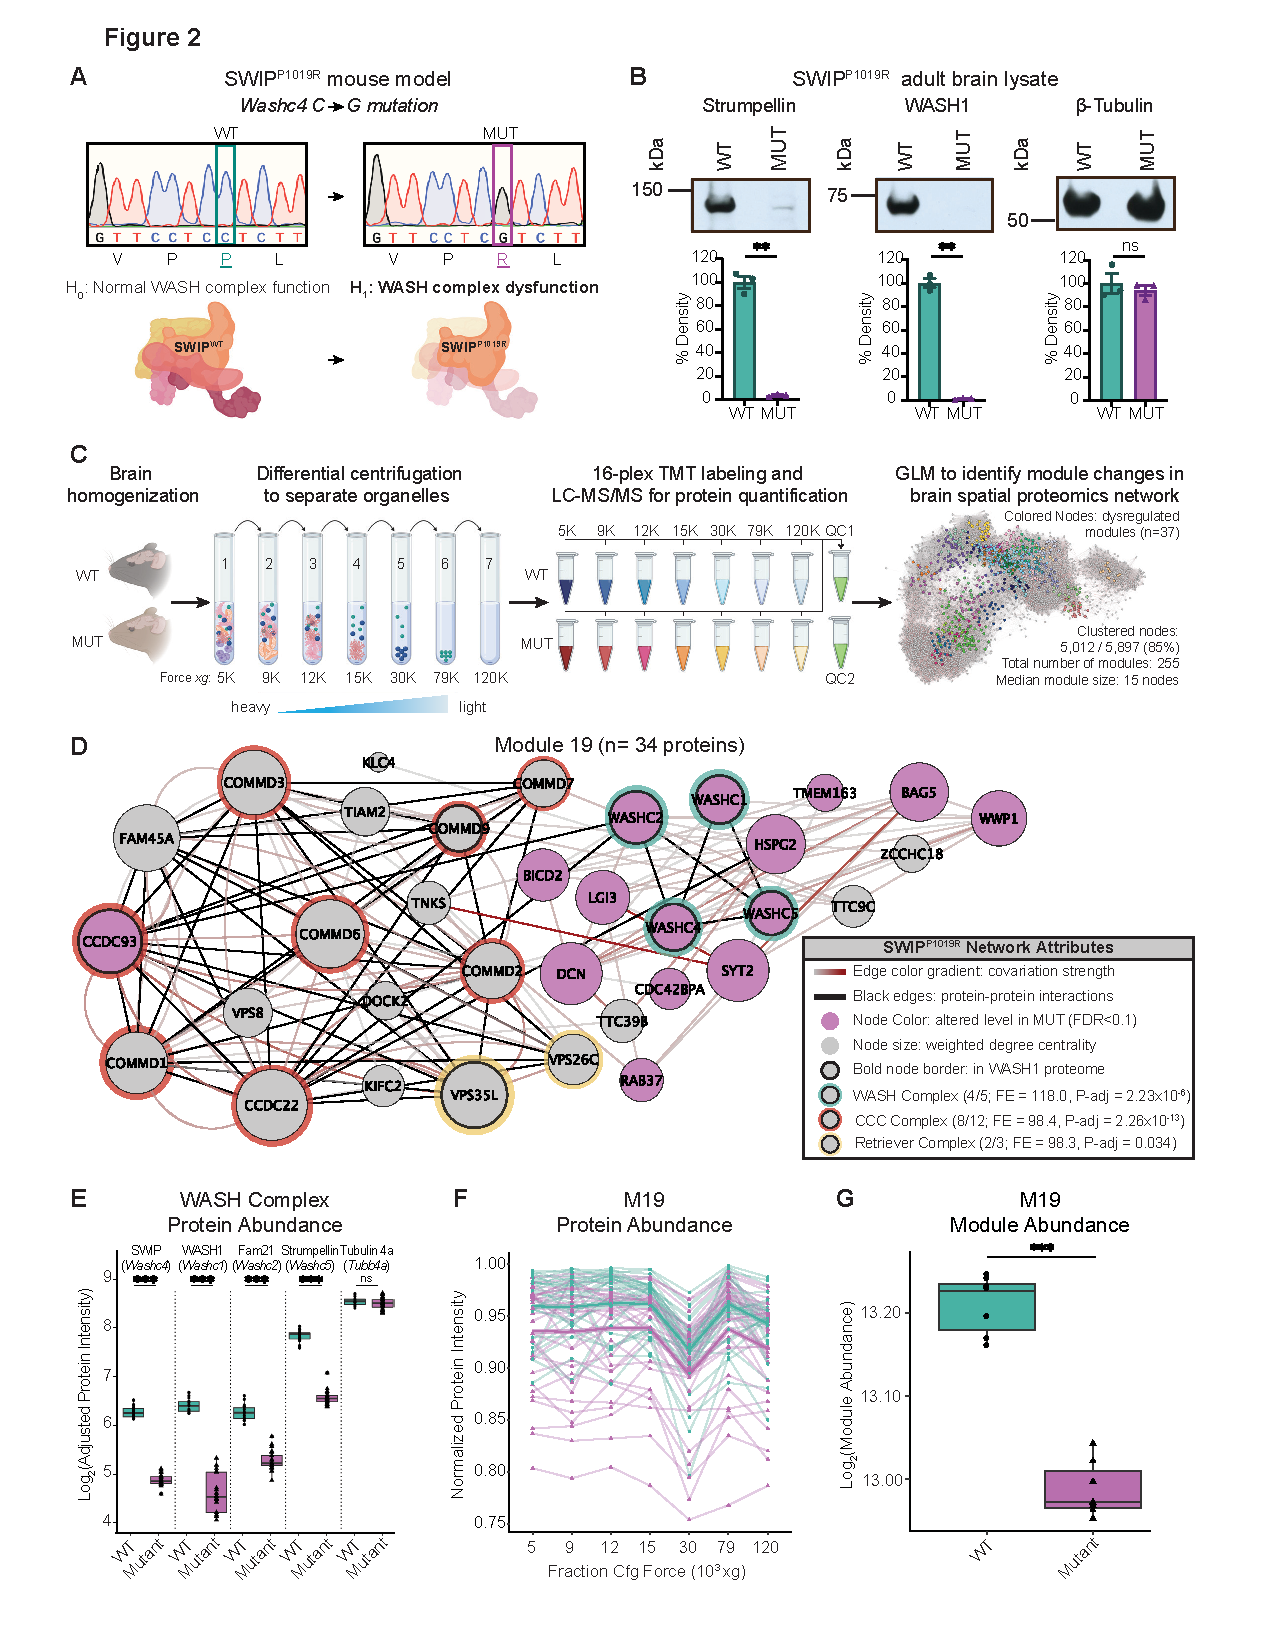
\includegraphics[height=0.5\linewidth, keepaspectratio]{Figure_01}
        \caption{\legend}
	\end{fullwidth}
\end{figure}
